%% Esempio per lo stile supsi
\documentclass[twoside]{supsistudent} 
\usepackage{graphicx}
\usepackage{subcaption}

% per settare noindent
\setlength{\parindent}{0pt}


% Crea un capitolo senza numerazione che pero` appare nell'indice %
\newcommand{\problemchapter}[1]{%
  \chapter*{#1}%
  \addcontentsline{toc}{chapter}{#1}%
\markboth{#1}{#1}
}

% Numerazione delle appendici secondo norma
\addto\appendix{
\renewcommand{\thesection}{\Alph{chapter}.\arabic{section}}
\renewcommand{\thesubsection}{\thesection.\arabic{subsection}}}

\setcounter{secnumdepth}{5} 	%per avere più livelli nei titoli
\setcounter{tocdepth}{5}		%per avere più livelli nell'indice


\titolo{DocTT --- Document Tagging Tool}
\studente{Cristian Spozio \vspace{1em}\\Denys Vitali}
\relatore{Daniele Puccinelli}
\correlatore{Salvatore Vanini}
\corso{Ingegeneria Informatica}
\modulo{M00009 - Progetto di diploma}
\anno{2019}



\begin{document}

\pagenumbering{alph}
\maketitle
\onehalfspacing
\frontmatter


\pagenumbering{roman}
\tableofcontents
\listoffigures					% Opzionale
\listoftables					% Opzionale

\newpage
\mainmatter
\pagenumbering{arabic}
\setcounter{page}{1}

\chapter*{Abstract}
\textit{DocTT} is a tagging tool which allows its users to tag text documents such as
press conferences or pitches. The tags take form in coloured rectangles
surrounding the text allowing a fast and easy visual recognition of a tag.
Tags are defined through a pre-uploaded tree by the user. The files involved
(document files and tree files) follow the XML standard and their parsing is 
managed by the tool.

\chapter*{Riassunto}
\lipsum[10]

\chapter{Introduzione}

\section{Struttura}

\textit{DocTT} si divide in 4 sezioni ognuna adibita ad una funzione specifica:
\begin{itemize}
  \item Home
  \item Document Upload
  \item Tree View
  \item Tree Upload
\end{itemize}

\subsection{Home}
La \textbf{Home} di \textit{DocTT} è la sezione in cui viene presentata la 
lista dei documenti caricati, dalla quale è possibile accedere ai documenti 
singoli e quindi alla loro modifica.

\begin{figure}[h!]
  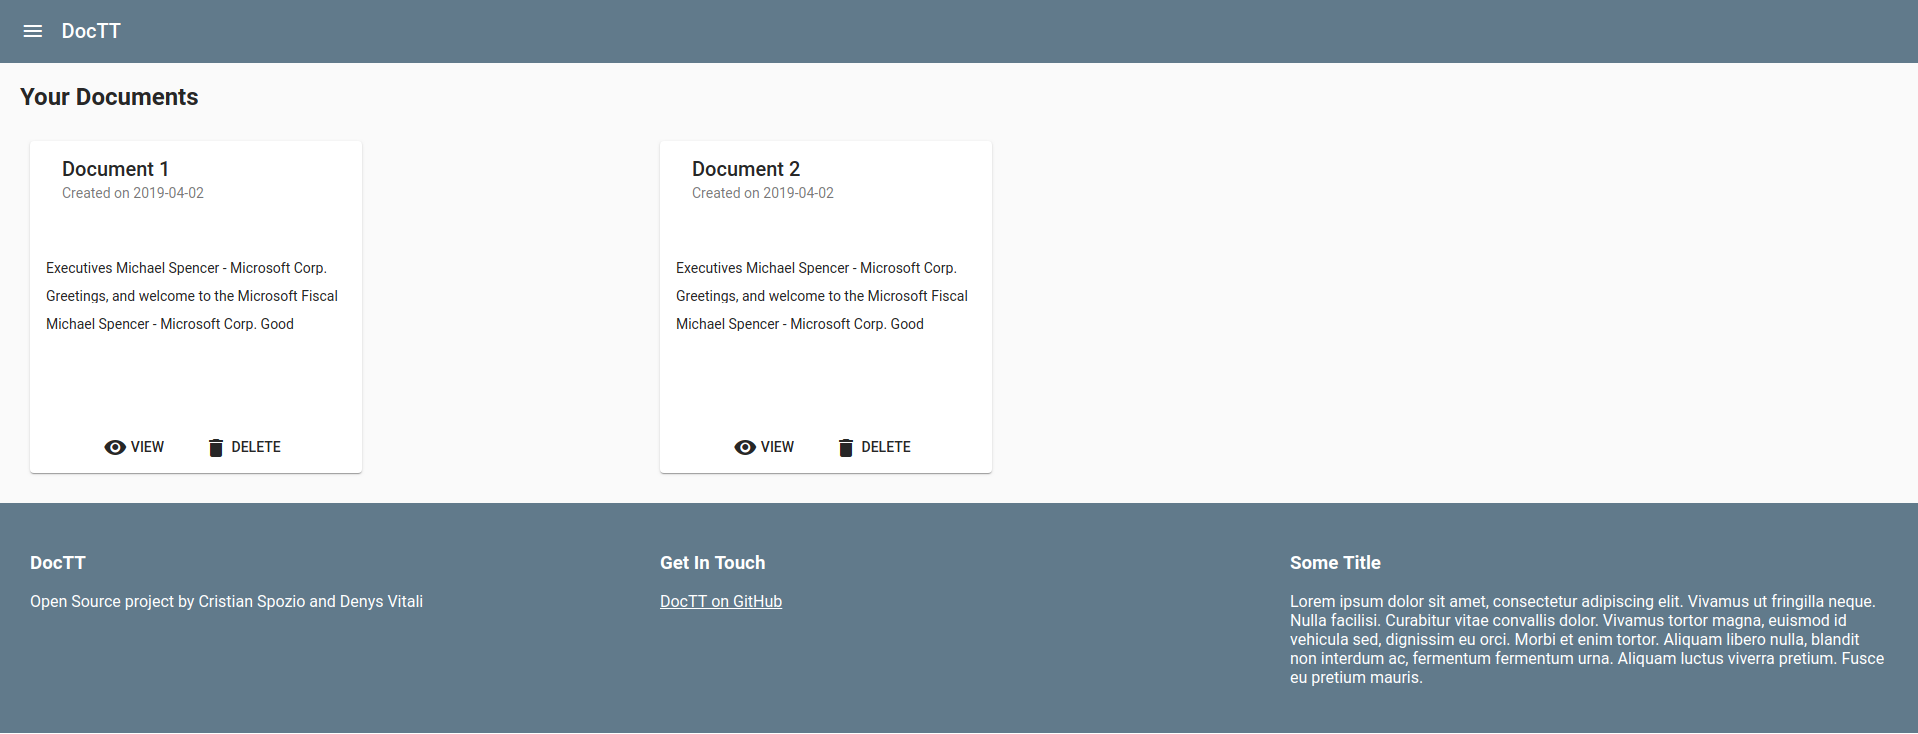
\includegraphics[width=\linewidth]{figures/home.png}
  \caption{Home section}
  \label{fig:home}
\end{figure}

\pagebreak

\subsection{Document Upload}
La sezione \textbf{Document Upload} di \textit{DocTT} è quella che permette
l'upload dei documenti da taggare ed il loro salvataggio nello storage del 
browser.

\begin{figure}[h!]
  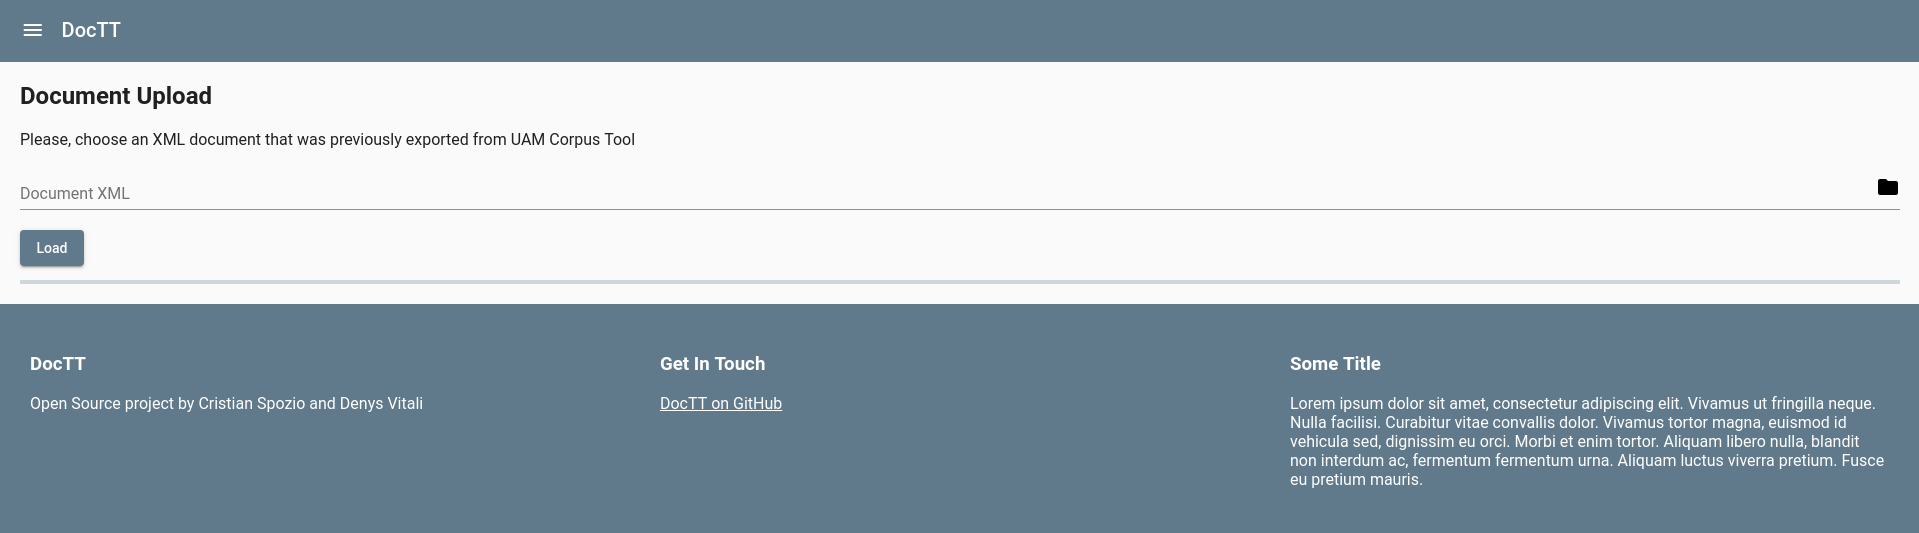
\includegraphics[width=\linewidth]{figures/docUpload.png}
  \caption{Document Upload section}
  \label{fig:docUpload}
\end{figure}

\subsection{Tree View}
La sezione \textbf{Tree View} di \textit{DocTT} è la parte che mostra l'albero
di tagging attualmente in uso come un elenco puntato espandibile per ogni
sottosezione presente.

\begin{figure}[h!]
  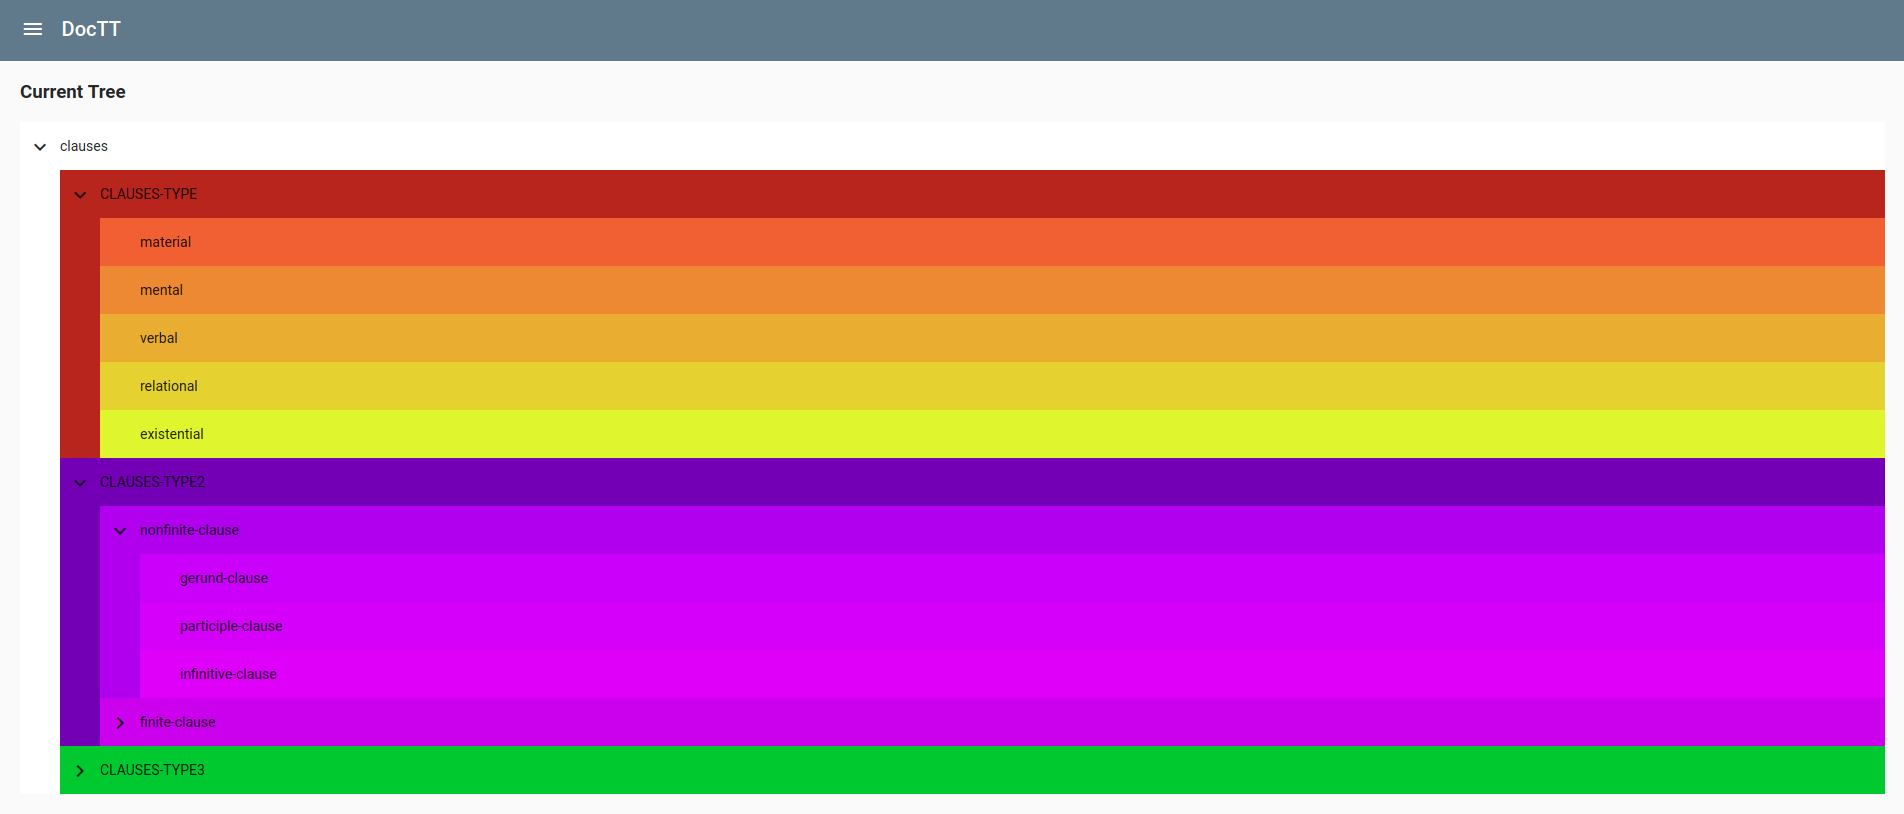
\includegraphics[width=\linewidth]{figures/treeView.png}
  \caption{Tree View section}
  \label{fig:treeView}
\end{figure}

\pagebreak

\subsection{Tree Upload}
La sezione \textbf{Tree Upload} di \textit{DocTT} è il componente che permette
l'upload dell'albero di tagging. Offre inoltre un'anteprima dell'albero 
attualmente in uso (nel caso ci fosse), secondo la stessa visualizzazione 
della sezione \textbf{Tree View}.
 
\begin{figure}[h!]
  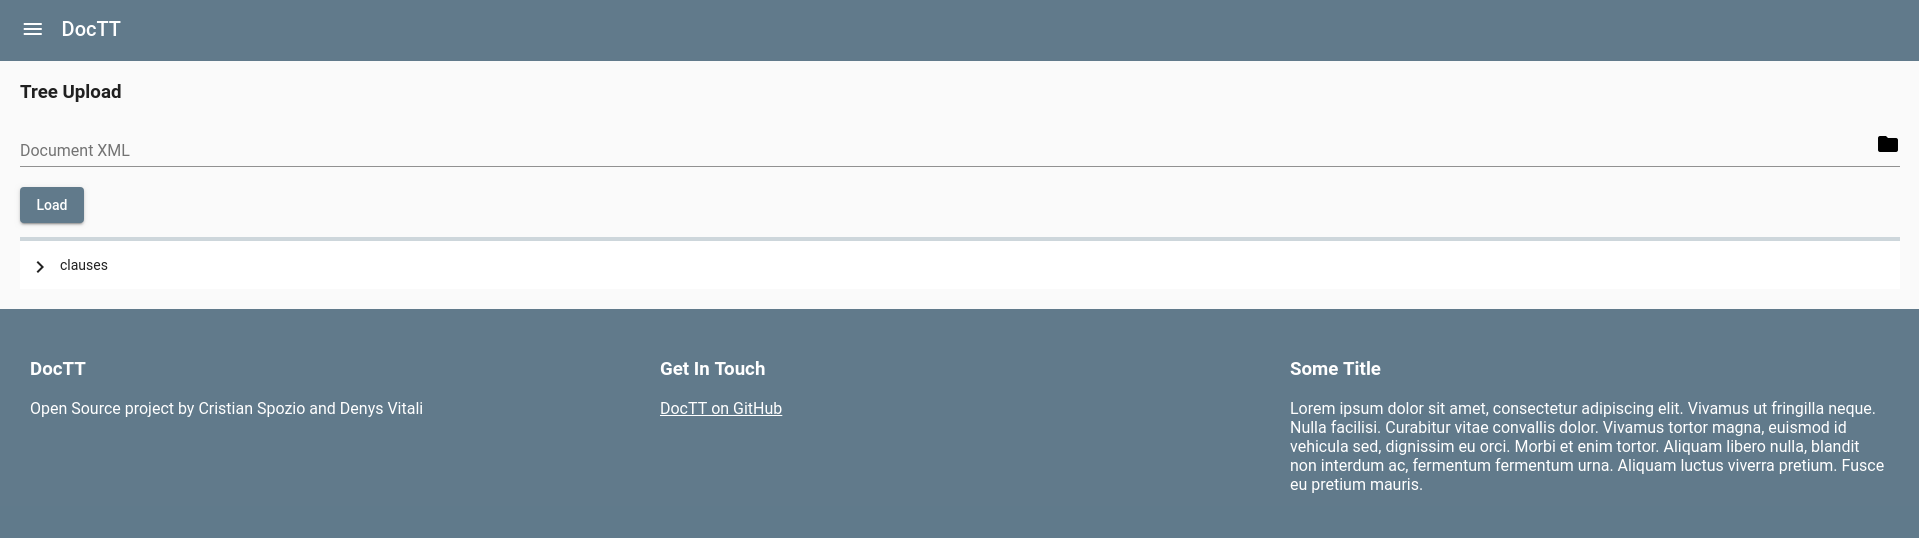
\includegraphics[width=\linewidth]{figures/treeUpload.png}
  \caption{Tree Upload section}
  \label{fig:treeUpload}
\end{figure}

\section{Tecnologie}
DocTT è stato sviluppato in \textbf{Angular}
\footnote{Angular : Framework per la creazione di UI in TypeScript}
secondo le direttive fornite dal relatore. È quindi stata divisa \textit{app}
nelle sottosezioni directives, models, modules, services e shared. I 
\textit{componenti Angular} sono stati quindi divisi in 3 parti: struttura, 
stile e funzione rispettivamente secondo i linguaggi \textbf{HTML5}, 
\textbf{SCSS} e \textbf{TypeScript}.

\chapter{Funzionamento}

\section{Processo di tagging}

Il processo di tagging può venire effettuato solo dopo il caricamento di un 
albero di tagging e dopo la selezione di un documento, operazioni eseguibili
nelle apposite sezioni del tool. 

\subsection{Floating menu}

La procedura effettiva di tagging viene effettuata selezionando del testo, al
completamento di questa operazione apparirà un menu alla fine della selezione,
contenente l'albero di tagging dal quale l'utente potrà andare a scegliere
quale tag attrubuire alla selezione.

\begin{figure}[h!]
  \centering
  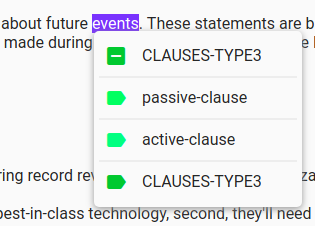
\includegraphics[width=7cm]{figures/floatingTag.png}
  \caption{Floating Tagging Menu}
  \label{fig:floatingTag}
\end{figure}

\pagebreak

\subsection{Nested tags}

Il tagging può essere effettuato a più livelli, quindi un tag (o più) possono
essere contenuti in un altro tag (o più).

\begin{figure}[h!]
  
\includegraphics[width=\linewidth]{figures/nestedTags.png}
  \caption{Nested Tags Example}
  \label{fig:nestedTags}
\end{figure}

\subsection{Tag removal}

I tag sono facilmente rimovibili semplicemente cliccando su di essi.

\begin{figure}[h!]
  \centering
  \begin{subfigure}[b]{0.4\linewidth}
    
\includegraphics[width=\linewidth]{figures/tagRemoval1.png}
    \caption{Before the click}
  \end{subfigure}
  \begin{subfigure}[b]{0.4\linewidth}
    
\includegraphics[width=\linewidth]{figures/tagRemoval2.png}
    \caption{After the click}
  \end{subfigure}
  \caption{Tag Removal Example}
  \label{fig:tagRemoval}
\end{figure}


%Citazione:
%\begin{quote}
%\lipsum[23]
%\end{quote}

%\lipsum[13]

%\begin{itemize}
%  \item Elemento A
%  \item Elemento B
%  \item Elemento C
%\end{itemize}

%\begin{itemize}
%  \item[-] Elemento A
%  \item[-] Elemento B
%  \item[-] Elemento C
%\end{itemize}
%
%\begin{enumerate}
%  \item Alpha
%  \item Beta
%  \item Gamma
%\end{enumerate}

%\lipsum[23]
%\section{Sezione}
%
%\lipsum[23]
%
%\subsection{Sotto sezione}
%
%Un po' di matematica: \newline
%
%\begin{math}
%\frac{n!}{k!(n-k)!} = {n \choose k}
%\end{math} \newline
%
%Un po' di matematica centrata:
%
%\begin{center}
%\begin{math}
%\frac{n!}{k!(n-k)!} = {n \choose k}
%\end{math}
%\end{center}
%
%Oppure con \$\$
%
%$$
%\frac{n!}{k!(n-k)!} = {n \choose k}
%$$
%
%Oppure anche direttamente nel testo ${1}\over{n}$ \\
%
%\lipsum[23]

\bibliographystyle{unsrt}
\bibliography{bibliografia}
\end{document}
